%% tags: [graph representations]
%% source: 2023-sp-redemption_midterm_02
\begin{prob}
    Let $A$ be the adjacency matrix of the graph shown below:

    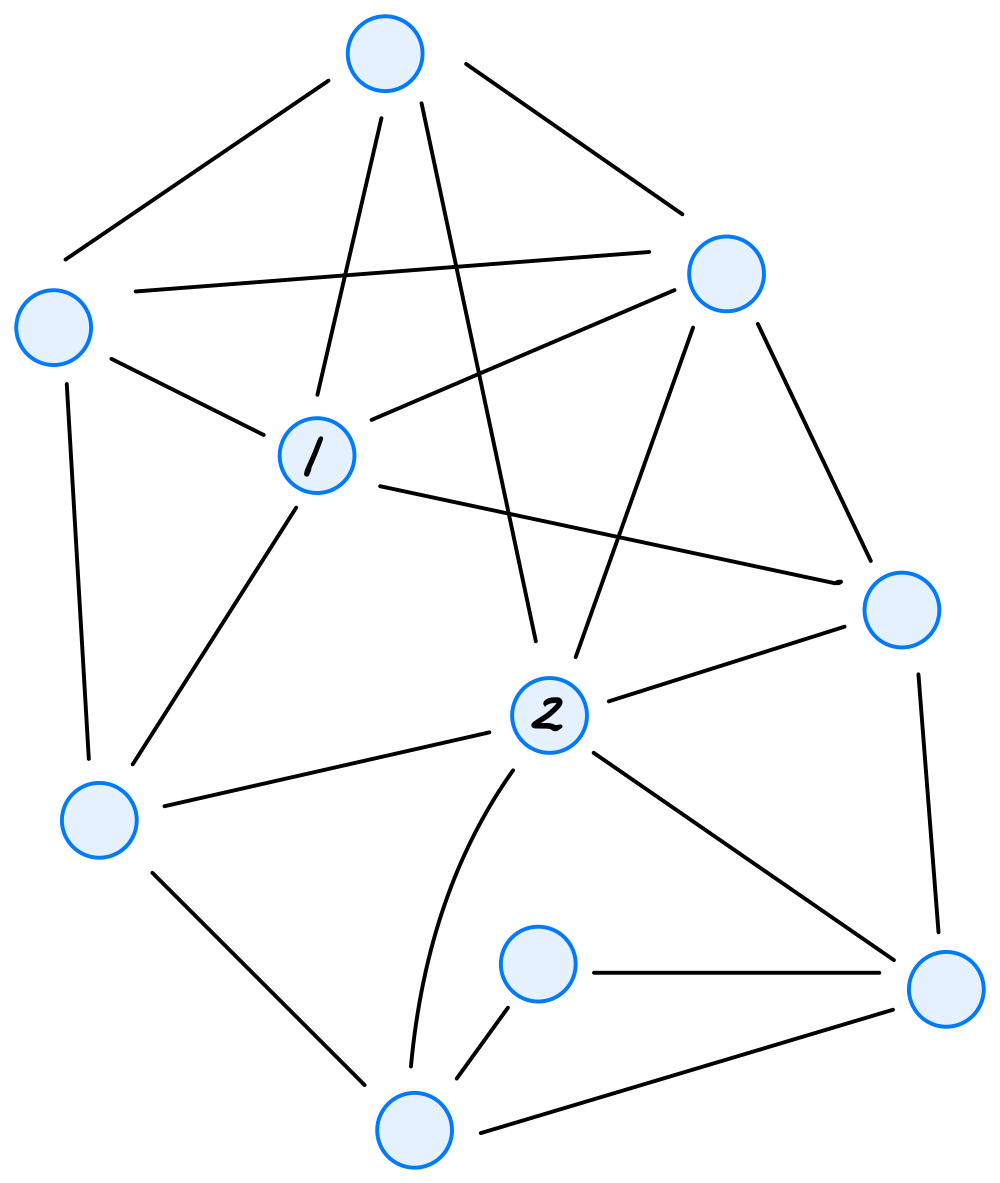
\includegraphics[width=.4\textwidth]{./graph.png}

    Let
    $\vec{a}^{(1)}$ be the first row of $A$ and
    $\vec{a}^{(2)}$ be the second row of $A$.
    What is $\vec{a}^{(1)} \cdot \vec{a}^{(2)}$?
    That is, what is the dot product between the first row of $A$ and the second row
    of $A$? Your answer should be in the form of a number.

    It may help to recall that the dot product between vectors $\vec x = (x_1,
    \ldots, x_d)^T$ and $\vec y = (y_1, \ldots, y_d)^T$ is equal to
    $x_1 y_1 + x_2 y_2 + \ldots + x_d y_d$.

    \begin{soln}
        4
    \end{soln}

\end{prob}
